\documentclass[12pt,a4paper]{article}
\usepackage[german]{babel}
\usepackage[T1]{fontenc}
\usepackage[utf8x]{inputenc}
\usepackage{url}
\usepackage{graphicx}
\usepackage{geometry}
\usepackage{amsfonts}
\usepackage{amsmath}
\usepackage{tabularx}
\usepackage{txfonts} %Times New Roman Font
\usepackage{titlesec} %Format der Headings ändern
\usepackage{hyperref}
\usepackage{comment}
\usepackage{listings}


\renewcommand{\thesection}{\arabic{section}.} %Nummerierung der Sections anpassen
\renewcommand{\labelenumi}{\alph{enumi})}  %Nummerierung der Listen anpassen
\titleformat{\section}{\large\bfseries}{\thesection}{0.5em}{} %Format der Section Überschrift ändern
\setlength{\parindent}{0pt} %Keine Einrückung bei neuen Paragraphen
\geometry{left=2.0cm,textwidth=17cm,top=2.5cm,textheight=23cm}

% Anpassen %
%%%%%%%%%%%%%%%%%%%%%%%%%%%%%%%%%%%%%
\newcommand{\student}{Daniel Pantjuskin-Moos\\ 108013248222 } % Namen eintragen
\newcommand{\partner}{Vincent König\\ 108011232630} % Matrikelnummer eintragen
\newcommand{\thirdone}{Max Mustermann\\ 108012345678}
\newcommand{\group}{D} % Gruppennummer eintragen
%%%%%%%%%%%%%%%%%%%%%%%%%%%%%%%%%%%%%

\newcommand{\hwheadtwo}{$ $
  \vspace{-2cm}
  
\noindent \student \qquad \qquad  Wireless Physical Layer Security Praktikum \hfill SS 2020 \\
\noindent \partner \\
%\noindent \thirdone \\  % einkommentieren, falls ihr eine 3er Gruppe seid
\noindent Gruppe:~\group\\
$ $

  
\begin{center}    
{\Large \bf Abgabe PHYSEC 2}
\end{center}
}

\begin{document}
\hwheadtwo

\section{FM-Empfänger}



 
\begin{figure}[hbt!]
\centering
	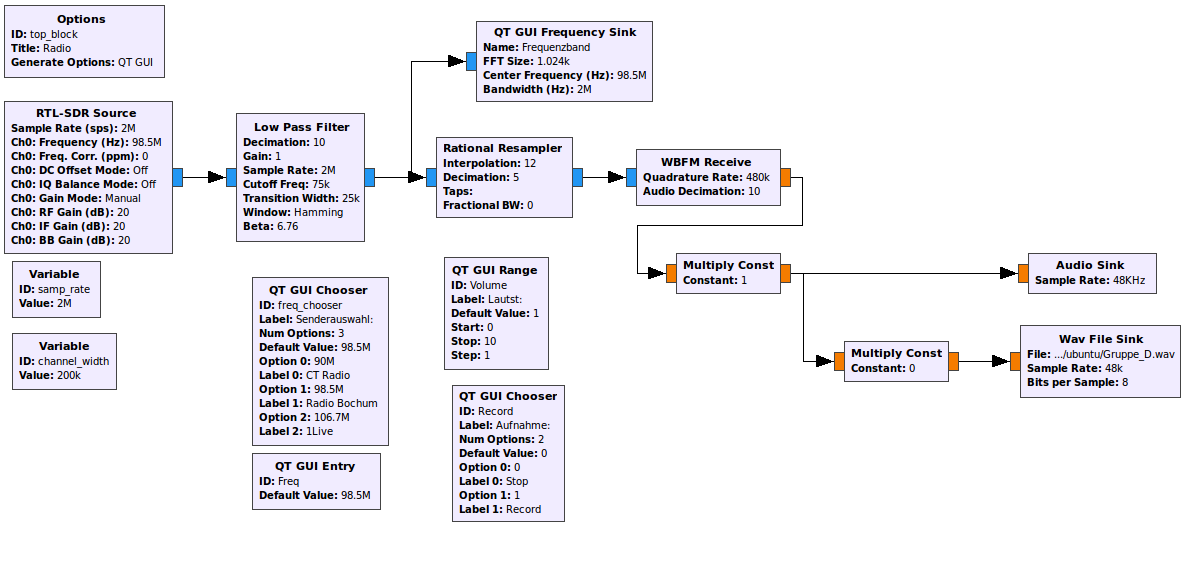
\includegraphics[width=1\textwidth ]
	{Bilder/Aufgabe1-gesamt-grc.png}
	\caption{Schaltung in GRC}
	\label{fig:Label1}
\end{figure}

Wie in Abbildung~\ref{fig:Label1} zu erkennen ist, wurden 
verschiedene Bausteine verwendet, die nun aufgezählt werden. 
Dabei wird auch darauf eingegangen, welche Aufgaben sie bewältigen.

\begin{itemize}
	\item \textit{Options}: Ermöglicht einzustellen, welche Art von 
	GUI, hier QT, verwendet werden soll
	\item \textit{RTL-SDR Source}: Es ermöglicht die Verarbeitung 
	von empfangenen Signalen, mithilfe von angeschlossener Hardware,
	hier \textit{HackRF}
	\item \textit{Variable} (oben und unten): Bequeme Steuerung der 
	Werte, die in Baublöcke einfließen 
	\item \textit{Low Pass Filter}: Dient zur Verfeinerung des 
	Signals durch Filtern. Laut 
	
	\href{https://youtu.be/TZmHgIPBLDo?t=1313}
	{Software Defined Radio with HackRF, Lesson 1: Welcome} 

	ist es Teil der Demodulation. Es dient als Vorbereitung der 
	eigentlichen Demodulation
	\item \textit{QT GUI Chooser} (links) und \textit{QT GUI Entry}:
	Dient zur Senderauswahl, oder genauer, der Frequenzauswahl
	\item \textit{QT Frequency Sink}: Visuelle Verdeutlichung des 
	Signals. Es zeigt die Wirkung des \textit{Low Pass Filters}
	\item \textit{Rational Resampler}: Da der \textit{Low Pass 
	Filter} nur eine ganzzahlige \textit{Decimation} unterstützt
	wird zusätzlich dieser \textit{Resampler} benötigt
	\item \textit{QT GUI Range} und \textit{Multiply Const} (links):
	Dient der Lautstärke-Einstellung
	\item \textit{GT GUI Chooser} (rechts), \textit{Multiply Const} 
	(rechts) und \textit{Wav File Sink}: Regelt die Aufnahme mit 
	\textit{Record} und \textit{Stop} des Empfangs als auch die 
	Abspeicherung als \textit{Gruppe\_D.wav} 
	\item \textit{WBFM Receive}: Der eigentliche Demodulierer laut
	 
	\href{https://youtu.be/TZmHgIPBLDo?t=1547}
	{Software Defined Radio with HackRF, Lesson 1: Welcome}.

	Es formt das Signal in Audio um	
\end{itemize}

Zusatz:\\
\textit{Samp\_rate} ist hier 2 Mio. Die 
\textit{Decimation} beim \textit{Low Pass Filter} ist 10:\\\\
$\frac{2 000 000}{10}= 200 000$\\\\
Der \textit{Rational Resampler} hat eine \textit{Interpolation} 
von 12 und eine \textit{Decimation} von 5:\\~\\
$200 000 * \frac{12}{5}= 480 000$\\\\
Der \textit{WBFM Receiver} hat eine \textit{Decimation} von 10:\\\\
$\frac{480 000}{10}= 48 000$\\~\\
48kHz ist eine gängige \textit{Sample Rate}, die von nahezu allen 
\textit{Soundcards} unterstützt wird.\\~\\

Hinweise:
\begin{itemize}
	\item Die Hyperlinks oben sind schon mit den passenden 
	Timestamps versehen
	\item Der von GRC ausgegebene Python2 Sourcecode 
	und die entsprechende .grc-Datei können 
	\href{https://mega.nz/file/Dgwz1TJK#Ij82qKY9ne4je0WJau5FlC7m422H0vi4gds5uQJ7J0s}
	{<hier>} runtergeladen werden
\end{itemize} 

Abbildung~\ref{fig:Label2} zeigt die fertige GUI. Oben lässt sich 
die Lautstärke einstellen. Ist der Slider ganz links, dann ist das 
Radio stumm. Darunter lässt sich mit \textit{Record} und 
\textit{Stop} die Aufnahme steuern. Bei \textit{Freq.} kann man 
die gewünschte Frequenz eingeben. Bei \textit{Senderauswahl} kann
man zu \textit{CT Radio}, \textit{Radio Bochum} und \textit{1Live}
schalten. \\\\
Es folgen danach die Einstellungen der wichtigsten Bauteile, 
die in  Abbildung~\ref{fig:Label1} zu sehen sind in Form 
von Screenshots.


\begin{figure}[hbt!]
\centering
	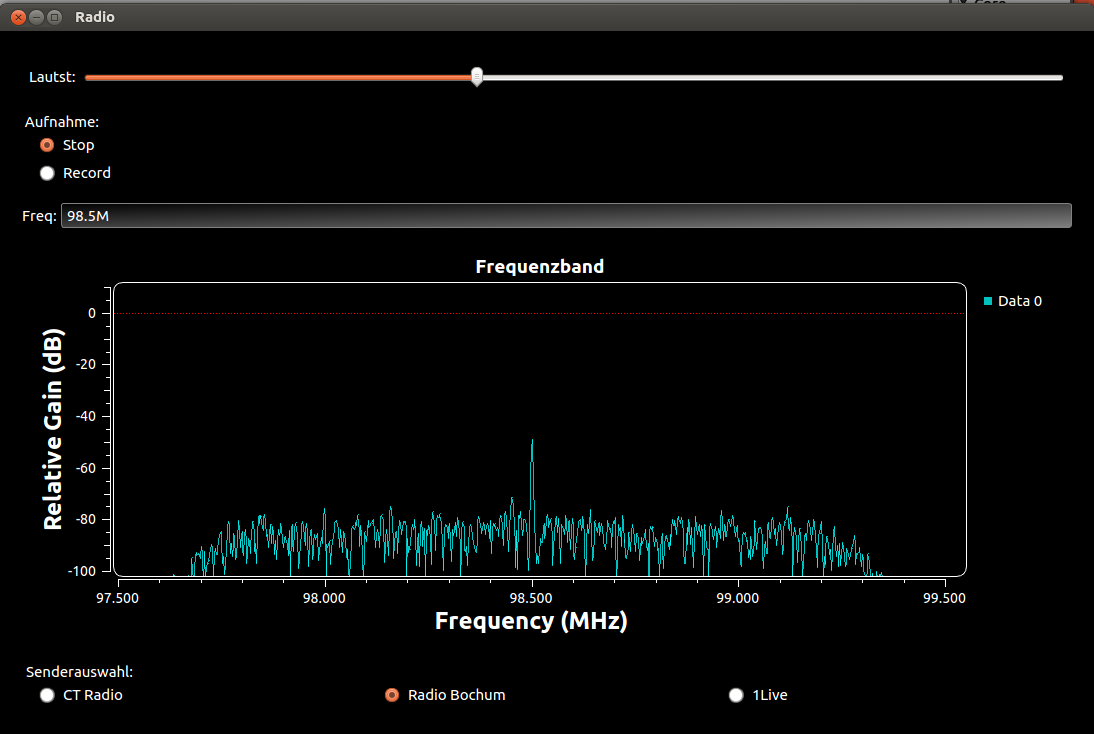
\includegraphics[width=0.9\textwidth ]
	{Bilder/Aufgabe1-gui.png}
	\caption{Fertige GUI}
	\label{fig:Label2}
\end{figure}


\begin{figure}[hbt!]
\centering
	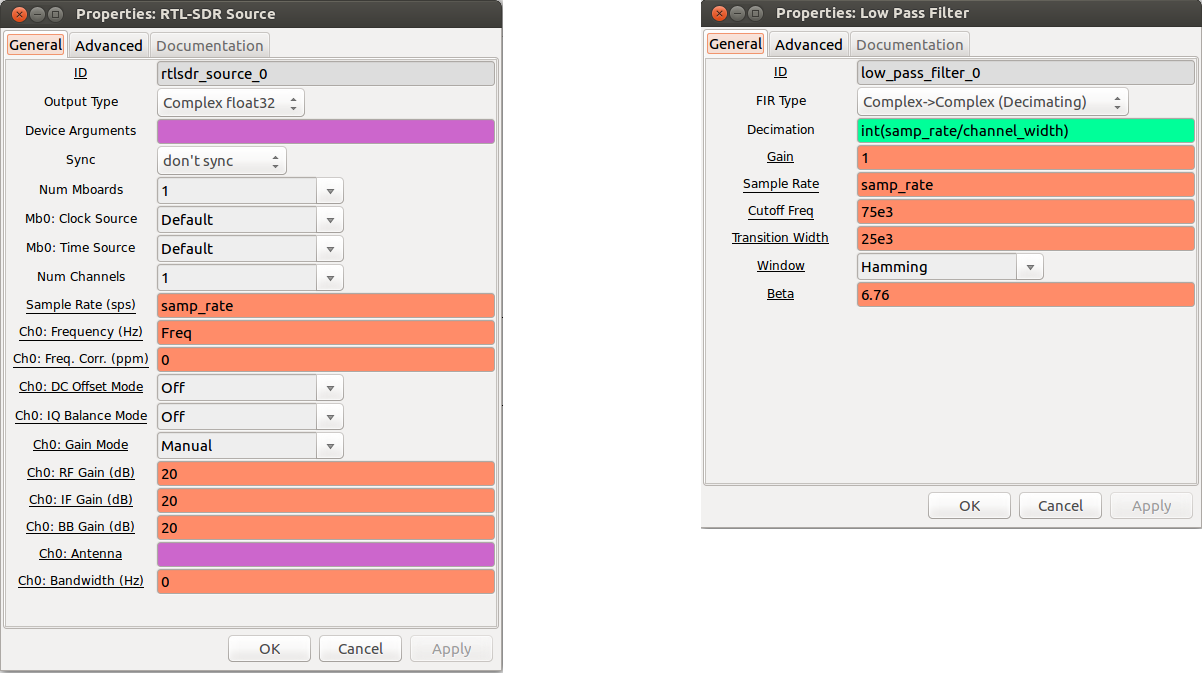
\includegraphics[width=0.9\textwidth ]
	{Bilder/Aufgabe1-properties1.png}
	%\caption{Bytes ASCII kodiert}
	\label{fig:Label3}
\end{figure}


\begin{figure}[hbt!]
\centering
	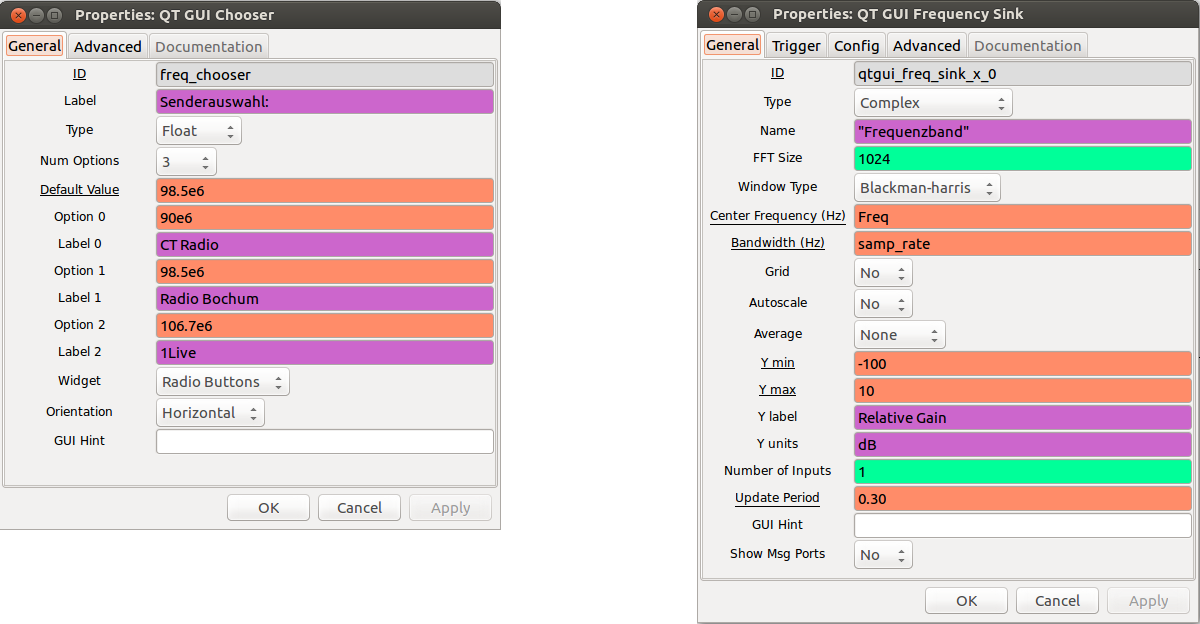
\includegraphics[width=0.9\textwidth ]
	{Bilder/Aufgabe1-properties2.png}
	%\caption{Bytes ASCII kodiert}
	\label{fig:Label4}
\end{figure}


\begin{figure}[hbt!]
\centering
	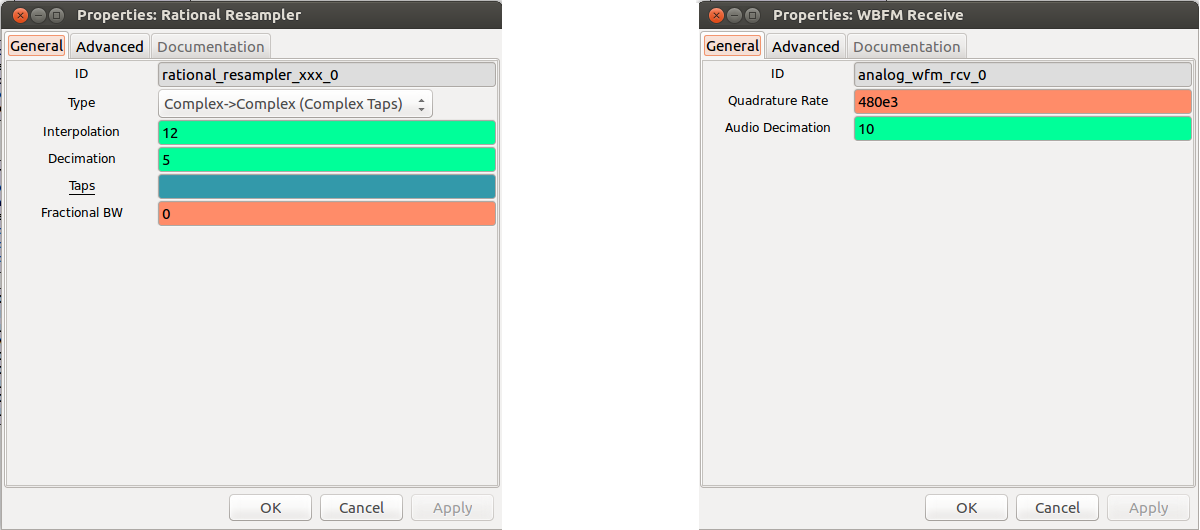
\includegraphics[width=0.9\textwidth ]
	{Bilder/Aufgabe1-properties3.png}
	%\caption{Bytes ASCII kodiert}
	\label{fig:Label5}
\end{figure}


\begin{figure}[hbt!]
\centering
	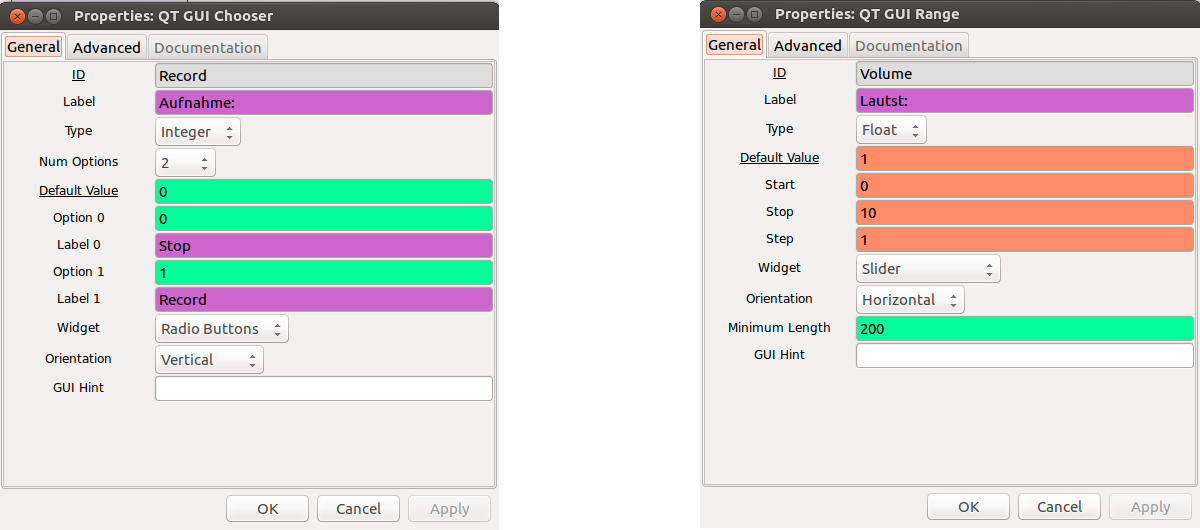
\includegraphics[width=0.9\textwidth ]
	{Bilder/Aufgabe1-properties4.png}
	%\caption{Bytes ASCII kodiert}
	\label{fig:Label6}
\end{figure}
\clearpage

\begin{figure}[hbt!]
\centering
	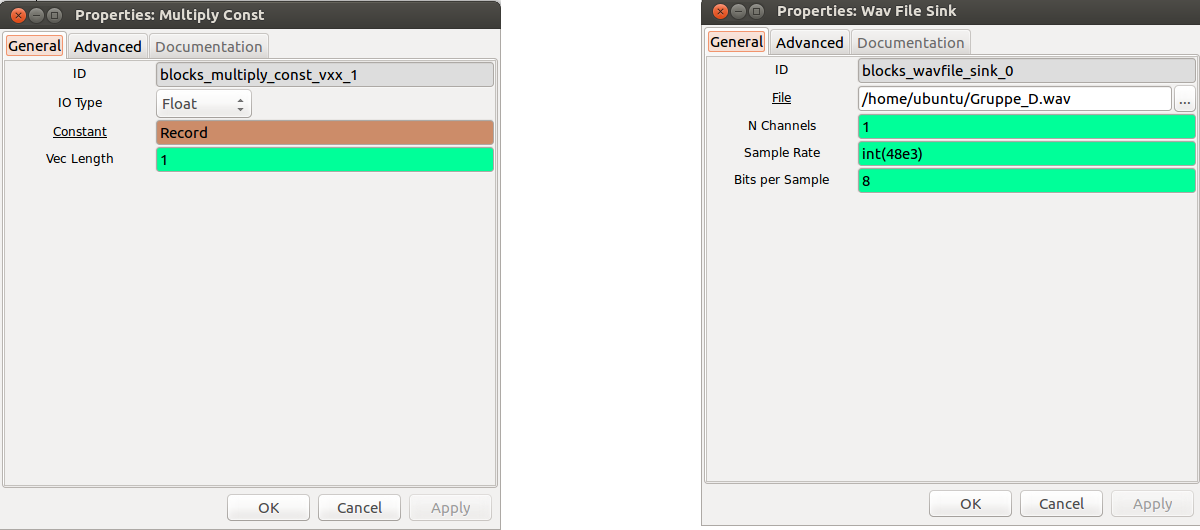
\includegraphics[width=0.9\textwidth ]
	{Bilder/Aufgabe1-properties5.png}
	%\caption{Bytes ASCII kodiert}
	\label{fig:Label7}
\end{figure}


\newpage
\section{Spectrum Spraying}
\begin{verbatim}
import scipy.ndimage as img
import numpy as np


def makeBinary(input_filename, output_filename='out.bin'):
	# Options for the FFT
	Fs = 1800000
	T_line = 0.005

	# Read input image
	image = img.imread(input_filename)

	# Set FFT size to be double the image size so that the
	# edge of the spectrum stays clear
	# preventing some bandfilter artifacts
	NFFT = 2*image.shape[1]

	# Repeat image lines until each one comes often enough to
	# reach the desired line time
	repetitions = int(np.ceil(T_line * Fs / NFFT))
	ffts = ((np.repeat(image[:, :, 0], repetitions, axis=0)/16.)**2.)/256.

	# Embed image in center bins of the FFT
	fftall = np.zeros((ffts.shape[0], NFFT))
	startbin = int(NFFT/4)
	fftall[:, startbin:(startbin+image.shape[1])] = ffts

	# Generate random phase vectors for the FFT bins, this is important to
	# prevent high peaks in the output
	# The phases won't be visible in the spectrum
	phases = 2*np.pi*np.random.rand(*fftall.shape)
	rffts = fftall * np.exp(1j*phases)

	# Perform the FFT per image line, then concatenate them to form the
	# final signal
	timedata = np.fft.ifft(np.fft.ifftshift(
		rffts, axes=1), axis=1)/np.sqrt(float(NFFT))
	linear = timedata.flatten()
	linear = linear / np.max(np.abs(linear))

	# Match the requirements
	res = np.zeros(2*linear.size, dtype=np.float32)
	res[0::2], res[1::2] = np.real(linear), np.imag(linear)

	# Get the Output
	res.tofile(output_filename)

	return


# Create the Signals
makeBinary('signal_kreis.png', 'signal_kreis.bin')
makeBinary('physec.png', 'physec.bin')

\end{verbatim}


\subsection*{• physec}

\begin{figure}[hbt!]
	\centering
		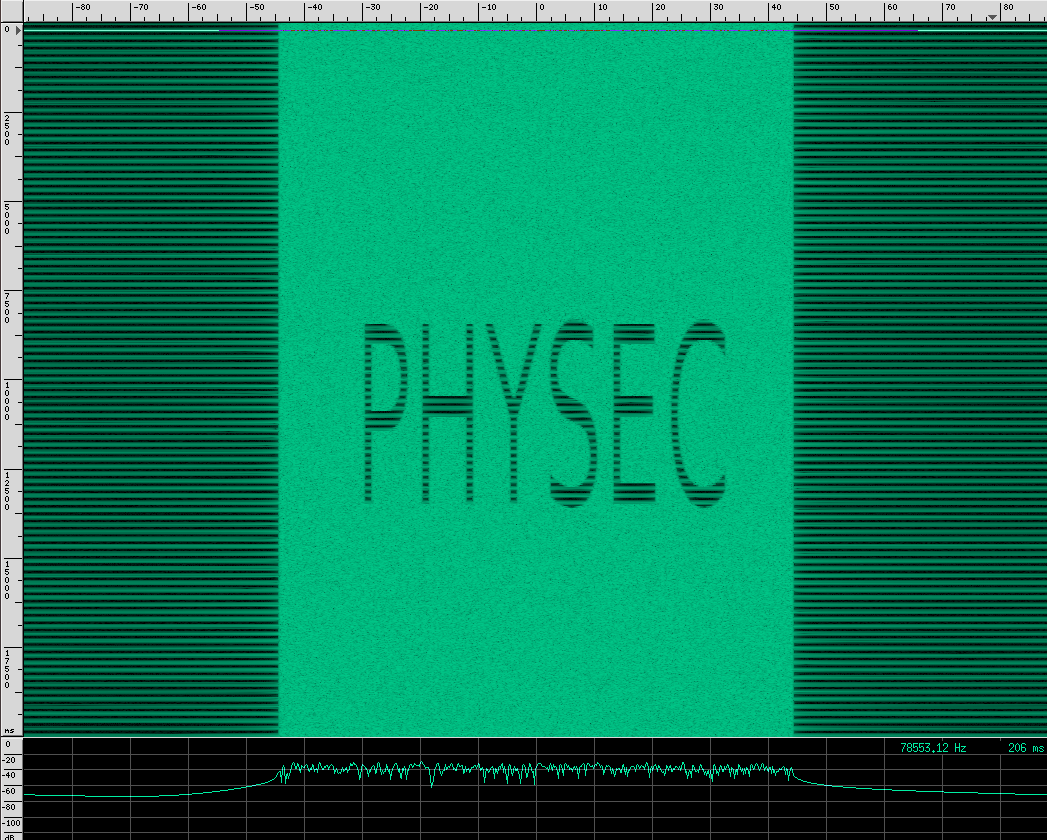
\includegraphics[width=1\textwidth ]
		{Bilder/A2_physec.png}
		\caption{physec.bin in Baudline}
		%\label{fig:Labelx}
\end{figure}



\newpage
\subsection*{• kreis}
%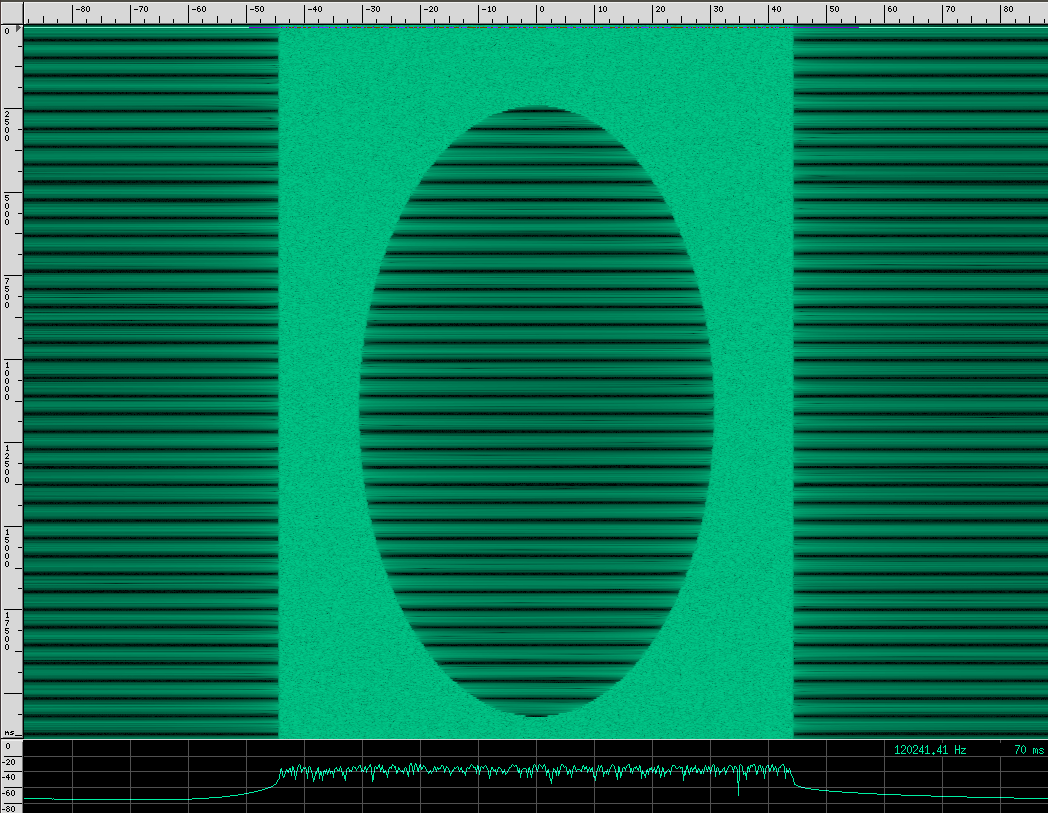
\includegraphics[width=0.85\textwidth ]{Bilder/A2_kreis.png}

\begin{figure}[hbt!]
	\centering
		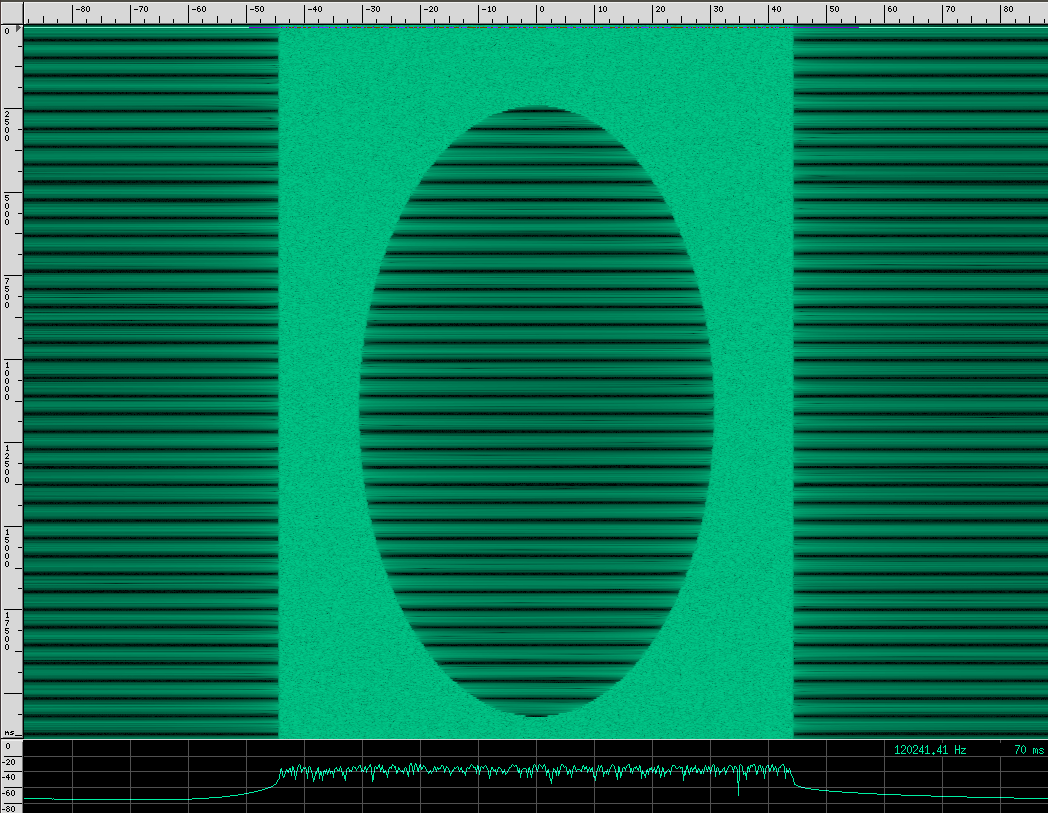
\includegraphics[width=1\textwidth ]
		{Bilder/A2_kreis.png}
		\caption{signal\_kreis.bin in Baudline}
		%\label{fig:Labelx}
\end{figure}
\clearpage

\section{Spectrum Sensing}

\subsection*{Komplettes Frequenzband}

\begin{figure}[hbt!]
	\centering
		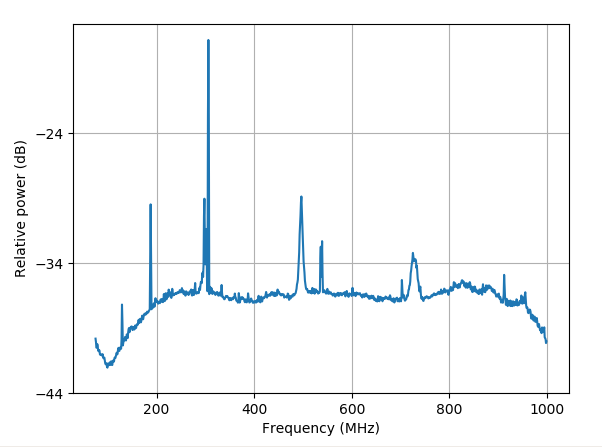
\includegraphics[width=1\textwidth ]
		{Bilder/A3_full_frequency_band.png}
		\caption{Frequenzband}
		%\label{fig:Labelx}
\end{figure}



\subsection*{Energy Detection}

\subsection*{Signale}

\subsection*{Unterschied zwischen RTL-SDR und HackRF}

\newpage
\section{Reading assignment}

\subsection*{a)} 
Siehe Seite 36 des Papers sollen damit \textit{resource 
depletion attacks} und \textit{masquerade attacks} 
abgewehrt werden.


\subsection*{b)} 
Siehe Seite 37 des Papers haben Signalprints die folgenden 
Eigenschaften:

\begin{itemize}
	\item Sie sind schwer zu \textit{spoofen} 
	\item Sie weisen eine starke Korrelation in Hinblick auf ihre 
	physikalische Umgebung auf
	\item Über mittlere Zeitdauern variieren sie nur leicht 
\end{itemize}


\subsection*{c)} 

\subsubsection*{Node Induction}
Da der Sender nur mithilfe des empfangenen Signalprints,
welches mit dem Referenz-Signalprints verglichen wird, 
identifiziert werden kann, muss das voraussetzen, dass 
das Referenz-Signalprint existiert. Falls jedoch eine 
Node zum ersten mal mit dem Netzwerk interagiert, fehlt 
logischerweise dieses Referenz-Signalprint, was das 
Identifizieren dieser Node nicht möglich macht. 
Wenn eine Node sich dem Netzwerk anschließen will, legt 
sie offen auf welchen Kanälen sie die restlichen 
Übertragungen senden wird. Die Empfänger stellen sich 
darauf ein und messen ihre jeweiligen RSSI Werte, die 
daraufhin über das Netzwerk verteilt werden. 

\subsubsection*{Frequent Hello Messages}
Aufgrund der kontinuierlichen Batterieentladung sinkt 
die Übertragunsstärke zunehmend, was zur Folge hat, 
dass die RSSI-Werte mit der Zeit abnehmen. 
Als Konsequenz wird der Vergleich der RSSI-Werte mit 
dem Signalprint nach einer gewissen Zeit beeinträchtigt 
und somit die Identifikation.
Im Allgemeinen kann die Entladungsrate nicht ohne Weiteres 
vom Empfänger vorrausgesagt werden, da es von der Ladung 
des Senders abhängt. Deshalb wird das regelmäßige Versenden 
von  \glqq hello\grqq \hspace{0.5mm} Packeten empfohlen.
Immer wenn ein Empfänger eine Übertragung eines Senders erhält, 
vergleicht dieser dann den empfangenen RSSI-Wert mit dem des 
Referenz-Signalprints. Erreicht die Differenz eine gewisse 
Größe, wird die Generierung eines neuen Referenz-Signalprints 
angefordert. Oft reicht der Verkehr von genuinen Übertragungen 
aus, aber ist das nicht der Fall müssen \glqq hello\grqq
\hspace{0.5mm}Packete übertragen werden zur erfolgreichen 
Verifizierung der RSSI-Werte.


\subsubsection*{Data Transmission}
Nicht jede Datenübertragung wird mithilfe eines Signalprints 
verifiziert. Je mehr Empfänger zusammenarbeiten um ein 
Signalprint zu generieren, desto höher die Verlässlichkeit 
des Signalprints. Es kann passieren, dass zu einem Zeitpunkt 
nicht genug Empfänger auf einen bestimmten Kanal eingestimmt 
sind um einen ausreichend verlässlichen Signalprint zu erhalten. 
Deshalb wird eine Methodik bestehend aus zwei Schritten verwendet:
\begin{itemize}
	\item Das Netzwerk hält Ausschau nach verdächtiger Aktivität
	\item Falls so eine Aktivität bemerkt wurde, stimmt das Netzwe 
	eine ausreichende Anzahl an Empfängern auf die entsprechenden 
	Kanäle ein und ein Signalprint wird erzeugt
\end{itemize}



%Als Beispiel für einen Hyperlink übrig gelassen
\begin{comment}
\href{https://www.pc-magazin.de/ratgeber/das-muessen-sie-ueber-lte-wissen-1277030.html}{(hier klicken)}
\end{comment}
\end{document}